\section{故障诊断实验与结果分析}
\label{sec:experiments_v8}

\subsection{引言}

前述章节分别完成了汽轮机系统健康状态建模、故障知识图谱构建以及KG-GCN故障诊断模型设计。本章在此基础上开展算例验证。本文总体研究对象为燃煤机组汽轮机热力系统，第三章构建的系统级知识图谱覆盖主通流、再热、抽汽回热及凝汽器冷端等主要设备和参数关系。考虑当前数据完整性和实验基础，选取超高压缸（VHP）作为代表性设备，对所提出的汽轮机系统KG-GCN故障诊断方法进行验证。

实验采用真实健康运行残差作为正常状态背景，并依据独立故障机理构造具有不同空间作用区域和时间演化形式的半物理故障场景。在相同数据条件下分别训练CNN、AE和KG-GCN，通过Accuracy、Precision、Recall、F1以及混淆矩阵比较三种方法的故障识别性能。

\subsection{研究对象及故障数据集}
\label{subsec:fault_dataset_v8}

VHP位于主蒸汽进入汽轮机后的首个主要膨胀设备，其状态既受到主蒸汽压力、温度、流量和调节阀等入口边界影响，又通过排汽与一次再热系统相连，并通过一级抽汽支路向1号高压加热器提供抽汽。因此，在VHP局部范围内同时存在汽缸本体、一级抽汽支路和再热接口等不同物理区域，可用于观察不同故障在参数空间中的传播差异。

第二章VHP健康状态模型对设备状态参数进行同步预测。完成状态点筛选后，最终选取24个状态参数用于故障诊断，主要包括VHP叶片级压力、排汽压力与温度、一级抽汽口压力与温度、一级抽汽逆止门前后温度、1号高压加热器入口抽汽压力与温度、一次低温再热接口温度以及VHP缸壁和内部蒸汽温度等。每个状态参数均保持固定DCS身份，并通过第三章设备--参数映射关系对应至VHP任务参数子图。

结合汽轮机通流部件退化、汽封泄漏机理、一级抽汽支路结构以及24个状态参数的可观测范围，设置正常状态和三类典型故障场景，如表~\ref{tab:fault_classes_v8}所示。

\begin{table}[htbp]
    \centering
    \caption{VHP故障诊断样本类别}
    \label{tab:fault_classes_v8}
    \begin{tabular}{p{1.0cm}p{4.2cm}p{5.2cm}p{3.3cm}}
        \toprule
        类别 & 故障场景 & 主要状态特征 & 主要作用区域 \\
        \midrule
        F0 & 正常状态 & 真实健康运行残差，不叠加故障响应 & 全部诊断节点 \\
        F1 & VHP通流部件侵蚀 & 有效通流面积及级组压力分布发生改变 & VHP本体、排汽及再热接口 \\
        F2 & 一级抽汽支路泄漏 & 抽汽蒸汽损失并引起下游抽汽状态变化 & 一级抽汽及1号高加入口 \\
        F3 & VHP汽封泄漏 & 无效蒸汽泄漏引起本体及排汽热力状态改变 & VHP本体、排汽及相关接口 \\
        \bottomrule
    \end{tabular}
\end{table}

健康背景数据取自2024年6月独立运行数据。利用第二章GRU健康状态模型计算24个状态参数的实测值与健康预测值之差，形成真实健康残差背景。对于第$k$类故障，第$n$个故障残差窗口表示为
\begin{equation}
R_{k,n}^{F}=R_n^{H}+a_{k,n}S_k\odot G_{k,n}+\epsilon_{k,n},
\end{equation}
式中：$R_n^{H}$为真实健康残差窗口；$S_k$为依据独立故障机理确定的空间响应模式；$a_{k,n}$为故障严重程度系数；$G_{k,n}$为故障随时间演化的动态函数；$\epsilon_{k,n}$为小幅随机扰动。

为避免模型记忆单一固定故障模板，不同样本随机设置故障发生时刻，并采用阶跃、斜坡或Sigmoid等不同时间演化形式。主实验中故障扰动强度在训练健康残差标准差的$2.0\sim3.0\sigma$范围内随机变化，该参数用于描述构造场景中的相对异常强度，不对应设备实际损伤百分比。

数据划分在故障样本构造之前完成。每连续5个自然日中，第1--3日作为训练集，第4日作为验证集，第5日作为测试集，任一60~min窗口均不跨越自然日边界。按照上述规则，训练集、验证集和测试集分别包含1712、556和560个样本，各类别保持均衡，样本分布见表~\ref{tab:fault_split_v8}。

\begin{table}[htbp]
    \centering
    \caption{故障诊断数据集样本分布}
    \label{tab:fault_split_v8}
    \begin{tabular}{lrrrr}
        \toprule
        数据集 & F0 & F1 & F2 & F3 \\
        \midrule
        训练集 & 428 & 428 & 428 & 428 \\
        验证集 & 139 & 139 & 139 & 139 \\
        测试集 & 140 & 140 & 140 & 140 \\
        \bottomrule
    \end{tabular}
\end{table}

当前机组尚缺少能够覆盖上述多类故障的完整现场故障记录，因此本章样本属于基于真实健康残差和独立故障机理构造的半物理故障场景。相关实验用于检验所提方法在该类机理一致构造条件下的诊断性能。

\subsection{实验设置与评估指标}
\label{subsec:experiment_setting_v8}

为比较不同特征学习方式的诊断效果，选取CNN和AE作为主要对比算法。CNN将多参数残差窗口作为参数--时间二维矩阵，通过局部卷积核提取故障特征；AE首先通过无监督重构获得低维潜在表示，再利用分类层完成故障识别；KG-GCN将状态残差加载至知识图谱对应参数节点，并根据参数邻接关系进行图卷积特征传播。三种模型采用完全相同的训练集、验证集和测试集。

KG-GCN参数节点数量为24，残差窗口长度为60，图卷积编码器包含2层GCN，节点隐藏特征维数为32。预训练阶段随机遮蔽15\%的残差位置，通过重构被遮蔽残差训练GCN编码器；完成预训练后固定图卷积编码器参数，利用带标签故障窗口训练全连接分类层。优化器采用AdamW，权重衰减为$1\times10^{-4}$。主要实验参数见表~\ref{tab:kg_setting_v8}。

\begin{table}[htbp]
    \centering
    \caption{KG-GCN模型主要实验参数}
    \label{tab:kg_setting_v8}
    \begin{tabular}{ll}
        \toprule
        参数 & 取值 \\
        \midrule
        参数节点数量 & 24 \\
        残差窗口长度 & 60 \\
        GCN层数 & 2 \\
        节点隐藏特征维数 & 32 \\
        Mask比例 & 15\% \\
        分类层隐藏维数 & 96 \\
        优化器 & AdamW \\
        权重衰减 & $1\times10^{-4}$ \\
        \bottomrule
    \end{tabular}
\end{table}

本文采用Accuracy、Precision、Recall和F1-score评价不同模型的故障诊断性能。对于第$k$类故障，Precision和Recall分别定义为
\begin{equation}
P_k=\frac{TP_k}{TP_k+FP_k},
\end{equation}
\begin{equation}
R_k=\frac{TP_k}{TP_k+FN_k},
\end{equation}
式中：$TP_k$为第$k$类故障被正确识别的样本数量；$FP_k$为其他类别被误判为第$k$类故障的样本数量；$FN_k$为第$k$类故障被误判为其他类别的样本数量。相应F1值为
\begin{equation}
F1_k=\frac{2P_kR_k}{P_k+R_k}.
\end{equation}
在多分类条件下，本文对各类别Precision、Recall和F1进行宏平均。整体准确率定义为
\begin{equation}
Accuracy=\frac{N_{correct}}{N_{all}},
\end{equation}
式中：$N_{correct}$为正确分类样本数量；$N_{all}$为测试样本总数。除上述指标外，进一步利用混淆矩阵分析各故障类别的具体识别情况。

\subsection{诊断结果与对比}
\label{subsec:results_v8}

表~\ref{tab:main_result_v8}给出了CNN、AE和KG-GCN三种模型在固定随机种子123下的故障诊断结果。KG-GCN的Accuracy为98.57\%，高于CNN的97.86\%和AE的95.54\%；其宏平均Precision、Recall和F1分别为98.60\%、98.57\%和98.58\%，四项指标均为三种模型中的最高值。CNN的Accuracy和F1分别为97.86\%和97.85\%，整体诊断精度较高；AE的四项指标约为95.5\%，低于另外两种方法。

\begin{table}[htbp]
    \centering
    \caption{CNN、AE和KG-GCN诊断结果对比}
    \label{tab:main_result_v8}
    \begin{tabular}{lcccc}
        \toprule
        模型 & Accuracy/\% & Precision/\% & Recall/\% & F1/\% \\
        \midrule
        CNN & 97.86 & 97.89 & 97.86 & 97.85 \\
        AE & 95.54 & 95.57 & 95.54 & 95.54 \\
        \textbf{KG-GCN} & \textbf{98.57} & \textbf{98.60} & \textbf{98.57} & \textbf{98.58} \\
        \bottomrule
    \end{tabular}
\end{table}

为考察结果对随机初始化的敏感程度，采用3组随机种子重复训练。CNN、AE和KG-GCN的平均Macro-F1分别为98.33\%$\pm$0.45\%、96.43\%$\pm$0.82\%和98.46\%$\pm$0.11\%。KG-GCN平均F1最高，同时标准差最小，说明其在不同随机初始化条件下保持了较稳定的诊断结果。图~\ref{fig:main_comparison_v8}进一步给出了三种模型Macro-F1的均值及标准差。

\begin{figure}[htbp]
    \centering
    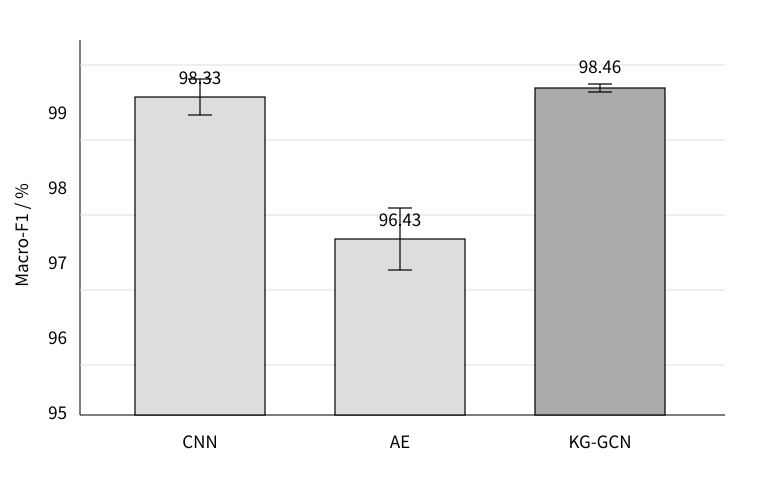
\includegraphics[width=0.78\textwidth]{figures/ch5/fig5_2_main_comparison.pdf}
    \caption{不同诊断模型三次重复实验Macro-F1比较}
    \label{fig:main_comparison_v8}
\end{figure}

为进一步观察各故障类别的误判方向，使用相同随机种子下的测试结果构造混淆矩阵，如图~\ref{fig:confusion_matrices_v8}所示。矩阵行表示真实类别，列表示预测类别。

\begin{figure}[htbp]
    \centering
    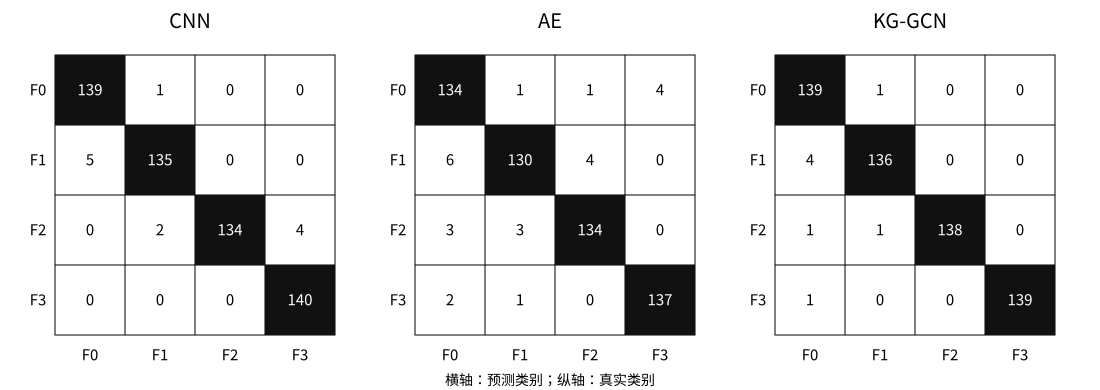
\includegraphics[width=0.99\textwidth]{figures/ch5/fig5_1_confusion_matrices.pdf}
    \caption{CNN、AE和KG-GCN故障诊断混淆矩阵}
    \label{fig:confusion_matrices_v8}
\end{figure}

由混淆矩阵可以看出，KG-GCN的分类结果最集中于主对角线，整体误诊数量最少。CNN共有12个测试样本发生误判，其中F2一级抽汽支路泄漏有4个样本被识别为F3 VHP汽封泄漏；AE共有25个样本发生误判，误判方向分散在F0、F1和F2等多个类别；KG-GCN仅有8个误判样本，其中F2有2个样本发生误判，F3仅有1个样本被识别为正常状态。

CNN主要依赖局部卷积核提取参数--时间矩阵中的局部动态特征。当不同故障在部分参数上的波动幅值或短时变化形态相近时，局部卷积特征难以显式表示这些参数在实际汽轮机结构中的位置差异。F2一级抽汽支路泄漏与F3 VHP汽封泄漏均可能在抽汽和排汽相关参数上形成状态变化，两类故障共享部分热力响应区域，因此CNN出现了F2向F3的类别交叉。

AE通过输入重构学习低维潜在表示，其优化目标主要描述多参数残差的整体数据分布。不同参数在潜在空间中的关联并不受到实际设备连接关系约束。当正常状态和不同故障的部分残差模式具有相近的重构特征时，分类层容易形成重叠的类别边界。由混淆矩阵可以看出，AE在多个类别之间均存在分散误判，与其总体F1低于CNN和KG-GCN的结果相对应。

KG-GCN在状态残差之外进一步利用了第三章知识图谱中的参数连接关系。对于F2故障，一级抽汽口、逆止门前后以及1号高压加热器入口构成连续的抽汽支路；对于VHP通流部件侵蚀和汽封泄漏，VHP本体压力、排汽状态以及一次再热接口形成不同的关联区域。GCN沿这些参数关系逐层聚合动态残差，使节点特征同时包含异常变化及其所在的热力结构位置。与只利用局部矩阵特征或潜在重构特征的模型相比，该结构信息有助于区分共享部分监测参数的故障类别，因此KG-GCN的混淆矩阵主对角线更加集中，整体误诊数量最低。

考虑故障标签数量有限时分类性能可能进一步下降，在主对比实验之后对掩码预训练进行补充验证。当分类阶段仅使用20\%带标签故障窗口时，直接从随机初始化训练KG-GCN的Macro-F1为94.48\%$\pm$0.93\%；采用残差窗口掩码预训练并固定GCN编码器后，Macro-F1提高至96.67\%$\pm$0.27\%，平均提高2.19个百分点。结果表明，在当前构造场景下，预训练能够利用不带类别标签的训练残差窗口提前学习参数之间的结构关联，并在故障标签减少时提供更稳定的特征表示。对应结果见图~\ref{fig:mask_ablation_v8}。

\begin{figure}[htbp]
    \centering
    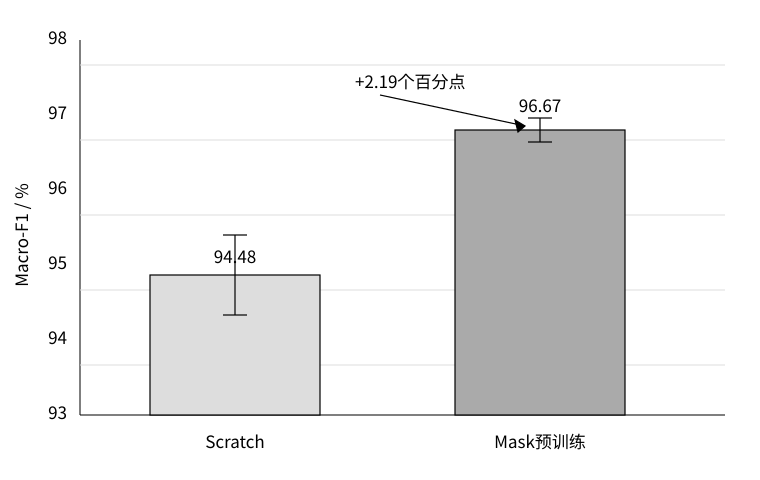
\includegraphics[width=0.76\textwidth]{figures/ch5/fig5_3_mask_ablation.pdf}
    \caption{20\%带标签样本下掩码预训练效果比较}
    \label{fig:mask_ablation_v8}
\end{figure}

\subsection{本章小结}

本章选取VHP作为代表性设备，对所提出的汽轮机系统KG-GCN故障诊断方法进行算例验证。基于2024年6月真实健康运行残差和独立故障机理构造正常状态、VHP通流部件侵蚀、一级抽汽支路泄漏和VHP汽封泄漏四类诊断样本，并按照自然日完成训练、验证和测试数据划分。在相同数据条件下，KG-GCN固定随机种子实验的Accuracy和F1分别达到98.57\%和98.58\%，均高于CNN和AE；混淆矩阵中KG-GCN的误诊样本数量最少。3组随机种子重复实验中，KG-GCN平均Macro-F1为98.46\%$\pm$0.11\%；在仅使用20\%带标签故障样本时，掩码预训练使Macro-F1提高2.19个百分点。上述结果说明，在本文构造的机理一致故障场景下，将状态监测残差信息与汽轮机参数知识关系进行融合，有助于提高多类别故障识别性能。当前结论仍需在后续现场故障记录或经校准的热力仿真数据上进一步验证。